\documentclass[11pt, a4paper]{article}
\usepackage[british]{babel}
\usepackage[utf8]{inputenc}
\usepackage{amsmath}
\usepackage{amssymb}
\usepackage{amsthm}
\usepackage{booktabs}
\usepackage{subfig}
\usepackage{bbold}
\usepackage[hidelinks]{hyperref}
\usepackage{graphicx}
\usepackage{xspace}
\usepackage{pgfplots}
\pgfplotsset{compat=newest}
%\usetikzlibrary{plotmarks}
%\usetikzlibrary{arrows.meta}
%\usepgfplotslibrary{patchplots}
%\usepackage{grffile}
\usepackage[section]{placeins}
\usepackage{tikz}
\usepackage{pgfgantt}
\usepackage{pdflscape}
\usepackage{siunitx}
\pgfplotsset{plot coordinates/math parser=false}

\newlength{\figwidth}
\setlength{\figwidth}{\textwidth}

\newcommand{\DUMUX}{DuMu$^\mathrm{x}$\xspace} %for convenience

\graphicspath{{img/}}

\theoremstyle{definition}
\newtheorem{defn}{Definition}

\title{\textbf{Channel flow with rough boundary}}
\author{Andrea Vescovini}
\date{\today}

\begin{document}
	\maketitle

\section{Introduction}
We want to test the behaviour of the TVD methods compared to the first order 
upwind method in the simulation of a channel flow with a wall boundary 
that is rough (i.e. not flat). Such a situation enhances the turbulence of the 
flow and the creation of turbulent eddies (\cite{pope}), so the benefit of 
using a higher order scheme should be noticeable. Moreover this is a situation 
that can be found in coupled problems with a free-flow and a porous-medium, 
because the interface between the two domains is usually rough 
(\cite{fetzer}).\\

\section{Test problem}
We solve the unsteady incompressible Navier-Stokes equations 
\eqref{eq:mass_bal} - \eqref{eq:mom_bal} over the channel domain $\Omega$. We 
impose a 
Dirichlet condition for the velocity \eqref{bc:in} at the inflow boundary 
$\Gamma_{in}$, no-slip conditions for the velocity \eqref{bc:w} at  the wall 
boundaries $\Gamma_w$, a zero-gradient conditions for the velocity 
\eqref{bc:outv} and a Dirichlet condition for the pressure \eqref{bc:outp} at 
the outflow boundary $\Gamma_{out}$. The problem is solved in the time interval 
$[0,T]$, starting from the initial conditions \eqref{ci:v}-\eqref{ci:p}. We 
choose $\varrho = \SI{1}{kg/m^3}$, $p_{ext} = \SI{1.1e5}{Pa}$ and $u_{in} = 
\SI{1}{m/s}$.

\begin{align}
\label{eq:mass_bal} \nabla \cdot
\mathbf{v} = 0 \quad &\text{in} \; \; \Omega \times [0, T]\\
\label{eq:mom_bal} \frac{\partial{(\varrho \mathbf{v}})}{\partial t} + \nabla 
\cdot (\varrho \mathbf{v} \mathbf{v^\mathrm{T}}) - \nabla \cdot (\mu (\nabla 
\mathbf{v} + \nabla \mathbf{v}^\mathrm{T})) + 
\nabla p = 0 \quad &\text{in} \; \; \Omega \times [0, T]\\
\label{bc:in} \mathbf{v} = [u_{in}, 0]^\mathrm{T} \quad &\text{on} \; \;
\Gamma_{in} \times [0, T]\\
\label{bc:w} \mathbf{v} = [0, 0]^\mathrm{T} \quad &\text{on} \; \; \Gamma_w 
\times [0, T]\\
\label{bc:outv} (\nabla \mathbf{v}) \mathbf{n} = [0, 0]^\mathrm{T}
\quad &\text{on} \; \; \Gamma_{out} \times [0,T]\\
\label{bc:outp} p = p_{ext} \quad &\text{on} \;\; \Gamma_{out} \times 
[0,T]\\
\label{ci:v} \mathbf{v} = [0, 0]^\mathrm{T} \quad &\text{in} \; \; \Omega, \; 
t=0\\
\label{ci:p} p = p_{ext} \quad &\text{in} \; \; \Omega, \; t=0
\end{align}

\subsection{First case}
First we set $\mu = \SI{5e-4}{\pascal\second}$, so that $Re = 2000$. The domain 
$\Omega$ 
is depicted in Figure \ref{fig:line_comp} and it is discretized using a mesh 
of \num{95x50} elements for its rectangular bounding box so that inside each 
small cavity there are \num{5x5} elements.
\begin{figure}[h]
	\centering
	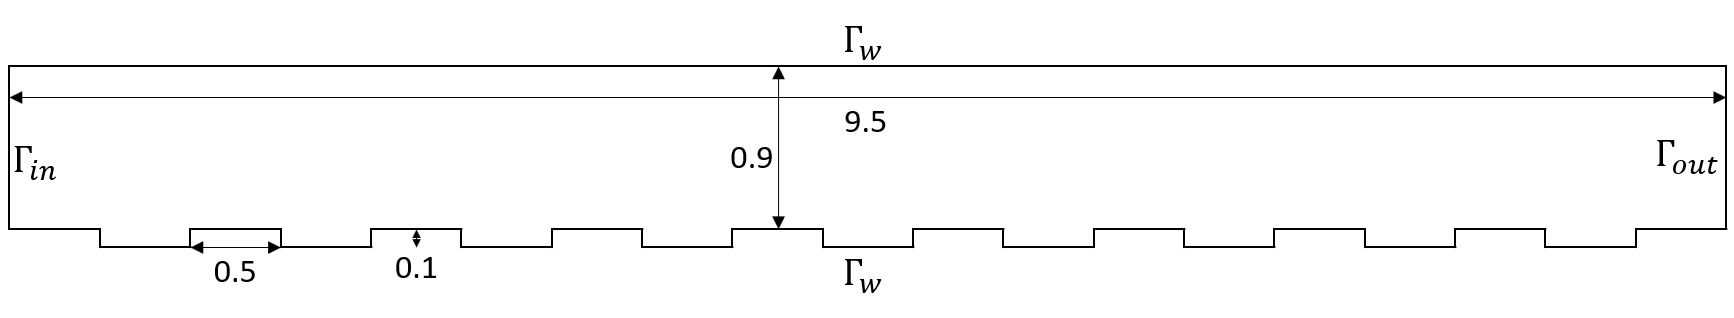
\includegraphics[width = \textwidth]{rough_domain.png}
	\caption{The domain $\Omega$ with a rough boundary made of small cavities.}
	\label{fig:rough_domain}
\end{figure}

The problem is solved over the time interval $[0, T] = [0, \SI{10}{s}]$, the 
initial 
$\Delta t$ is equal to \SI{0.005}{s}, then it is adapted according to the 
convergence 
of the Newton method at the previous time-step, with a maximum length of 
\SI{0.1}{s}.
A reference solution is computed over a mesh of \num{570x300} elements, 
employing the upwind scheme.

In Figure \ref{fig:line_comp} the magnitude of the velocity along a section of 
the channel at $x=\SI{8.75}{m}$ at the last time step is reported. From the 
plot we 
can see that the 
solution obtained using the TVD methods matches the reference solution, while 
the upwind one is slightly shifted towards the upper part of the channel. In 
Table \ref{tab:err} it is reported the $L^2$ error along the section between 
the different methods and the better behaviour of the TVD methods is confirmed.
From the plot we can also observe that even if the cavities are small there is 
a recirculation of the fluid inside them. 

\begin{figure}[h]
	\centering
	% This file was created by matlab2tikz.
%
\definecolor{mycolor1}{rgb}{0.00000,0.44700,0.74100}%
\definecolor{mycolor2}{rgb}{0.85000,0.32500,0.09800}%
\definecolor{mycolor3}{rgb}{0.92900,0.69400,0.12500}%
\definecolor{mycolor4}{rgb}{0.49400,0.18400,0.55600}%
%
\begin{tikzpicture}

\begin{axis}[%
width=0.951\roughwidth,
height=0.75\roughheight,
at={(0\roughwidth,0\roughheight)},
scale only axis,
xmin=0,
xmax=1,
xlabel={$y$ [m]},
ymin=0,
ymax=1.25,
ylabel={Velocity magnitude [m/s]},
axis background/.style={fill=white},
legend style={at={(0.5,0.03)}, anchor=south, legend cell align=left, align=left}
]
\addplot [color=mycolor1, mark size=1.5pt, mark=x, mark options={solid, mycolor1}, line width=0.75pt]
  table[row sep=crcr]{%
0	0\\
0.01	0.0293662\\
0.03	0.050586\\
0.05	0.0374104\\
0.07	0.00830816\\
0.09	0.0878588\\
0.11	0.203537\\
0.13	0.350154\\
0.15	0.504986\\
0.17	0.648407\\
0.19	0.773425\\
0.21	0.879108\\
0.23	0.965875\\
0.25	1.0347\\
0.27	1.08726\\
0.29	1.12581\\
0.31	1.15286\\
0.33	1.17097\\
0.35	1.18249\\
0.37	1.18938\\
0.39	1.19321\\
0.41	1.19513\\
0.43	1.19595\\
0.45	1.19618\\
0.47	1.19615\\
0.49	1.19606\\
0.51	1.19602\\
0.53	1.19608\\
0.55	1.19627\\
0.57	1.19661\\
0.59	1.19708\\
0.61	1.1977\\
0.63	1.19842\\
0.65	1.19918\\
0.67	1.19986\\
0.69	1.20024\\
0.71	1.19994\\
0.73	1.19831\\
0.75	1.19437\\
0.77	1.18669\\
0.79	1.17327\\
0.81	1.15154\\
0.83	1.11834\\
0.85	1.07018\\
0.87	1.00343\\
0.89	0.914856\\
0.91	0.802051\\
0.93	0.663892\\
0.95	0.500819\\
0.97	0.314904\\
0.99	0.109749\\
1	0\\
};
\addlegendentry{Upwind}

\addplot [color=mycolor2, mark size=1.5pt, mark=x, mark options={solid, mycolor2}, line width=0.75pt]
  table[row sep=crcr]{%
0	0\\
0.01	0.0271697\\
0.03	0.0500789\\
0.05	0.0401093\\
0.07	0.00567534\\
0.09	0.0811925\\
0.11	0.199174\\
0.13	0.35443\\
0.15	0.52202\\
0.17	0.675188\\
0.19	0.804904\\
0.21	0.91139\\
0.23	0.996051\\
0.25	1.06075\\
0.27	1.10807\\
0.29	1.14103\\
0.31	1.16275\\
0.33	1.17616\\
0.35	1.18381\\
0.37	1.1877\\
0.39	1.18933\\
0.41	1.18969\\
0.43	1.18942\\
0.45	1.18894\\
0.47	1.18845\\
0.49	1.18804\\
0.51	1.18779\\
0.53	1.1877\\
0.55	1.18779\\
0.57	1.18804\\
0.59	1.18848\\
0.61	1.18909\\
0.63	1.18985\\
0.65	1.19073\\
0.67	1.19161\\
0.69	1.19229\\
0.71	1.1924\\
0.73	1.19132\\
0.75	1.18802\\
0.77	1.181\\
0.79	1.16815\\
0.81	1.14675\\
0.83	1.11359\\
0.85	1.06512\\
0.87	0.997859\\
0.89	0.908818\\
0.91	0.795828\\
0.93	0.657971\\
0.95	0.495791\\
0.97	0.311428\\
0.99	0.10845\\
1	0\\
};
\addlegendentry{Van Leer}

\addplot [color=mycolor3, mark size=1.5pt, mark=x, mark options={solid, mycolor3}, line width=0.75pt]
  table[row sep=crcr]{%
0	0\\
0.01	0.0272093\\
0.03	0.0494723\\
0.05	0.0389859\\
0.07	0.00595636\\
0.09	0.0812851\\
0.11	0.198804\\
0.13	0.353914\\
0.15	0.5204\\
0.17	0.672249\\
0.19	0.801321\\
0.21	0.907555\\
0.23	0.992249\\
0.25	1.05727\\
0.27	1.10509\\
0.29	1.13867\\
0.31	1.16106\\
0.33	1.17513\\
0.35	1.18335\\
0.37	1.18771\\
0.39	1.18968\\
0.41	1.19029\\
0.43	1.19022\\
0.45	1.18987\\
0.47	1.18946\\
0.49	1.18912\\
0.51	1.18891\\
0.53	1.18887\\
0.55	1.18899\\
0.57	1.18928\\
0.59	1.18974\\
0.61	1.19035\\
0.63	1.19112\\
0.65	1.19197\\
0.67	1.19282\\
0.69	1.19344\\
0.71	1.19347\\
0.73	1.19226\\
0.75	1.18881\\
0.77	1.18163\\
0.79	1.16863\\
0.81	1.14714\\
0.83	1.11395\\
0.85	1.06554\\
0.87	0.998402\\
0.89	0.90948\\
0.91	0.796585\\
0.93	0.658719\\
0.95	0.496437\\
0.97	0.311872\\
0.99	0.108614\\
1	0\\
};
\addlegendentry{Min-Mod}

\addplot [color=mycolor4, line width=0.75pt]
  table[row sep=crcr]{%
0	0\\
0.00166667	0.00492427\\
0.005	0.0138838\\
0.00833333	0.0219483\\
0.0116667	0.0291114\\
0.015	0.0353663\\
0.0183333	0.0407062\\
0.0216667	0.0451241\\
0.025	0.0486134\\
0.0283333	0.051167\\
0.0316667	0.0527786\\
0.035	0.0534416\\
0.0383333	0.0531503\\
0.0416667	0.0518985\\
0.045	0.0496806\\
0.0483333	0.0464911\\
0.0516667	0.042324\\
0.055	0.037174\\
0.0583333	0.0310358\\
0.0616667	0.0239061\\
0.065	0.0157914\\
0.0683333	0.00678684\\
0.0716667	0.00421506\\
0.075	0.0150977\\
0.0783333	0.0273447\\
0.0816667	0.0407005\\
0.085	0.0551595\\
0.0883333	0.0707355\\
0.0916667	0.0874415\\
0.095	0.105279\\
0.0983333	0.124233\\
0.101667	0.144291\\
0.105	0.165438\\
0.108333	0.187646\\
0.111667	0.210875\\
0.115	0.23507\\
0.118333	0.260158\\
0.121667	0.286047\\
0.125	0.312628\\
0.128333	0.33978\\
0.131667	0.367367\\
0.135	0.395245\\
0.138333	0.42327\\
0.141667	0.451298\\
0.145	0.479192\\
0.148333	0.506829\\
0.151667	0.534103\\
0.155	0.560921\\
0.158333	0.587212\\
0.161667	0.612919\\
0.165	0.638002\\
0.168333	0.662436\\
0.171667	0.686204\\
0.175	0.7093\\
0.178333	0.731723\\
0.181667	0.753476\\
0.185	0.774566\\
0.188333	0.795\\
0.191667	0.814784\\
0.195	0.833928\\
0.198333	0.852438\\
0.201667	0.870321\\
0.205	0.887585\\
0.208333	0.904234\\
0.211667	0.920276\\
0.215	0.935716\\
0.218333	0.950561\\
0.221667	0.964818\\
0.225	0.978495\\
0.228333	0.991598\\
0.231667	1.00414\\
0.235	1.01612\\
0.238333	1.02756\\
0.241667	1.03847\\
0.245	1.04885\\
0.248333	1.05871\\
0.251667	1.06808\\
0.255	1.07696\\
0.258333	1.08537\\
0.261667	1.09332\\
0.265	1.10082\\
0.268333	1.10789\\
0.271667	1.11454\\
0.275	1.12079\\
0.278333	1.12664\\
0.281667	1.13213\\
0.285	1.13725\\
0.288333	1.14203\\
0.291667	1.14648\\
0.295	1.15062\\
0.298333	1.15445\\
0.301667	1.158\\
0.305	1.16127\\
0.308333	1.16429\\
0.311667	1.16706\\
0.315	1.1696\\
0.318333	1.17192\\
0.321667	1.17404\\
0.325	1.17597\\
0.328333	1.17771\\
0.331667	1.17929\\
0.335	1.18071\\
0.338333	1.18198\\
0.341667	1.18311\\
0.345	1.18412\\
0.348333	1.18501\\
0.351667	1.18579\\
0.355	1.18647\\
0.358333	1.18706\\
0.361667	1.18757\\
0.365	1.188\\
0.368333	1.18836\\
0.371667	1.18866\\
0.375	1.1889\\
0.378333	1.18908\\
0.381667	1.18923\\
0.385	1.18933\\
0.388333	1.18939\\
0.391667	1.18942\\
0.395	1.18942\\
0.398333	1.1894\\
0.401667	1.18935\\
0.405	1.18928\\
0.408333	1.1892\\
0.411667	1.18911\\
0.415	1.189\\
0.418333	1.18888\\
0.421667	1.18876\\
0.425	1.18863\\
0.428333	1.18849\\
0.431667	1.18836\\
0.435	1.18822\\
0.438333	1.18808\\
0.441667	1.18794\\
0.445	1.1878\\
0.448333	1.18766\\
0.451667	1.18753\\
0.455	1.1874\\
0.458333	1.18727\\
0.461667	1.18715\\
0.465	1.18703\\
0.468333	1.18691\\
0.471667	1.1868\\
0.475	1.1867\\
0.478333	1.1866\\
0.481667	1.18651\\
0.485	1.18642\\
0.488333	1.18634\\
0.491667	1.18626\\
0.495	1.18619\\
0.498333	1.18613\\
0.501667	1.18607\\
0.505	1.18601\\
0.508333	1.18597\\
0.511667	1.18593\\
0.515	1.18589\\
0.518333	1.18586\\
0.521667	1.18584\\
0.525	1.18582\\
0.528333	1.18581\\
0.531667	1.1858\\
0.535	1.1858\\
0.538333	1.18581\\
0.541667	1.18582\\
0.545	1.18584\\
0.548333	1.18586\\
0.551667	1.18589\\
0.555	1.18593\\
0.558333	1.18597\\
0.561667	1.18602\\
0.565	1.18607\\
0.568333	1.18613\\
0.571667	1.18619\\
0.575	1.18626\\
0.578333	1.18634\\
0.581667	1.18642\\
0.585	1.18651\\
0.588333	1.1866\\
0.591667	1.1867\\
0.595	1.18681\\
0.598333	1.18692\\
0.601667	1.18703\\
0.605	1.18716\\
0.608333	1.18729\\
0.611667	1.18742\\
0.615	1.18756\\
0.618333	1.18771\\
0.621667	1.18786\\
0.625	1.18802\\
0.628333	1.18819\\
0.631667	1.18835\\
0.635	1.18853\\
0.638333	1.18871\\
0.641667	1.18889\\
0.645	1.18908\\
0.648333	1.18927\\
0.651667	1.18947\\
0.655	1.18967\\
0.658333	1.18987\\
0.661667	1.19007\\
0.665	1.19028\\
0.668333	1.19048\\
0.671667	1.19068\\
0.675	1.19089\\
0.678333	1.19108\\
0.681667	1.19128\\
0.685	1.19147\\
0.688333	1.19165\\
0.691667	1.19182\\
0.695	1.19197\\
0.698333	1.19212\\
0.701667	1.19224\\
0.705	1.19235\\
0.708333	1.19243\\
0.711667	1.19249\\
0.715	1.19252\\
0.718333	1.19251\\
0.721667	1.19246\\
0.725	1.19237\\
0.728333	1.19223\\
0.731667	1.19204\\
0.735	1.19178\\
0.738333	1.19146\\
0.741667	1.19107\\
0.745	1.19059\\
0.748333	1.19003\\
0.751667	1.18937\\
0.755	1.1886\\
0.758333	1.18772\\
0.761667	1.18671\\
0.765	1.18557\\
0.768333	1.18428\\
0.771667	1.18283\\
0.775	1.18122\\
0.778333	1.17942\\
0.781667	1.17743\\
0.785	1.17523\\
0.788333	1.17282\\
0.791667	1.17016\\
0.795	1.16726\\
0.798333	1.16409\\
0.801667	1.16064\\
0.805	1.15689\\
0.808333	1.15283\\
0.811667	1.14845\\
0.815	1.14372\\
0.818333	1.13862\\
0.821667	1.13315\\
0.825	1.12728\\
0.828333	1.12101\\
0.831667	1.1143\\
0.835	1.10714\\
0.838333	1.09953\\
0.841667	1.09143\\
0.845	1.08284\\
0.848333	1.07374\\
0.851667	1.06411\\
0.855	1.05394\\
0.858333	1.04321\\
0.861667	1.0319\\
0.865	1.02002\\
0.868333	1.00753\\
0.871667	0.994433\\
0.875	0.980713\\
0.878333	0.96636\\
0.881667	0.951363\\
0.885	0.935712\\
0.888333	0.919401\\
0.891667	0.90242\\
0.895	0.884765\\
0.898333	0.866428\\
0.901667	0.847407\\
0.905	0.827698\\
0.908333	0.807298\\
0.911667	0.786206\\
0.915	0.764423\\
0.918333	0.74195\\
0.921667	0.718789\\
0.925	0.694943\\
0.928333	0.670418\\
0.931667	0.645219\\
0.935	0.619353\\
0.938333	0.592828\\
0.941667	0.565653\\
0.945	0.537839\\
0.948333	0.509397\\
0.951667	0.48034\\
0.955	0.45068\\
0.958333	0.420433\\
0.961667	0.389615\\
0.965	0.358241\\
0.968333	0.326328\\
0.971667	0.293895\\
0.975	0.260961\\
0.978333	0.227546\\
0.981667	0.193668\\
0.985	0.15935\\
0.988333	0.124612\\
0.991667	0.0894758\\
0.995	0.0539638\\
0.998333	0.0180982\\
1	0\\
};
\addlegendentry{Reference}
\addplot [color=black, dashed, line width=0.75pt]
  table[row sep=crcr]{%
0.1	0\\
0.1 1.25\\
};
\end{axis}
\end{tikzpicture}%
	\caption{Velocity magnitude at $x=\SI{8.75}{m}$ and $t=\SI{10}{s}$ at $Re = 
	2000$}
	\label{fig:line_comp}
\end{figure}

\begin{figure}[h]
	\centering
	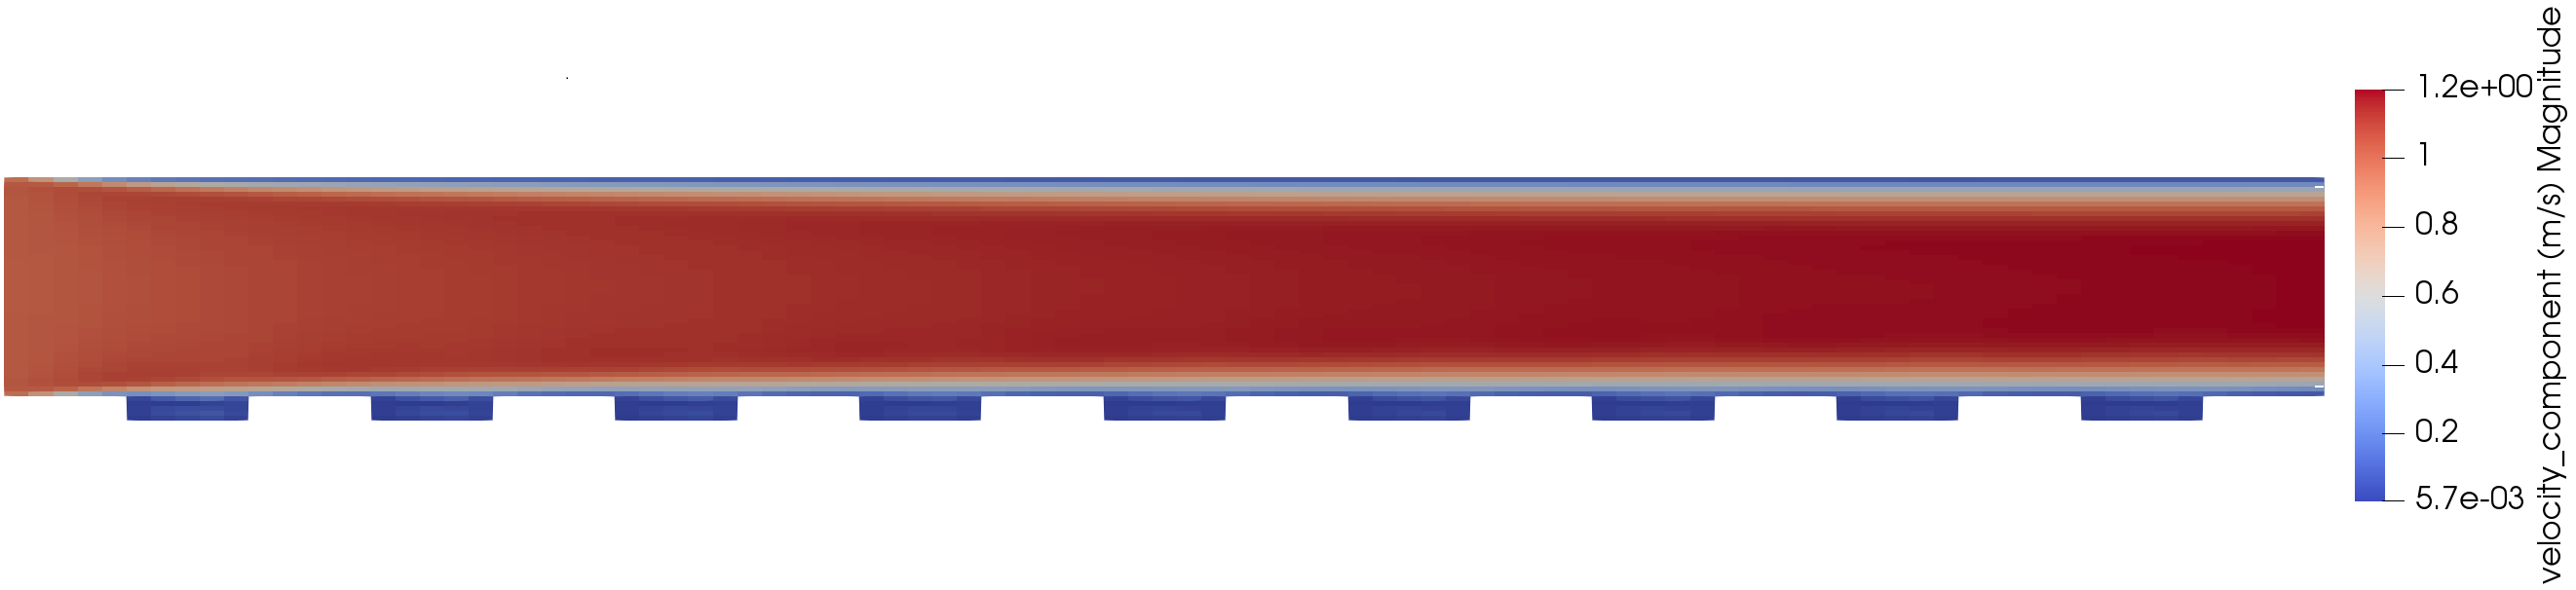
\includegraphics[width=\textwidth]{rough_channel_vl}
	\caption{Velocity magnitude at $t=\SI{10}{s}$, $Re=2000$, Van Leer method.}
	\label{fig:cha_vl}
\end{figure}

\begin{figure}[h]
	\centering
	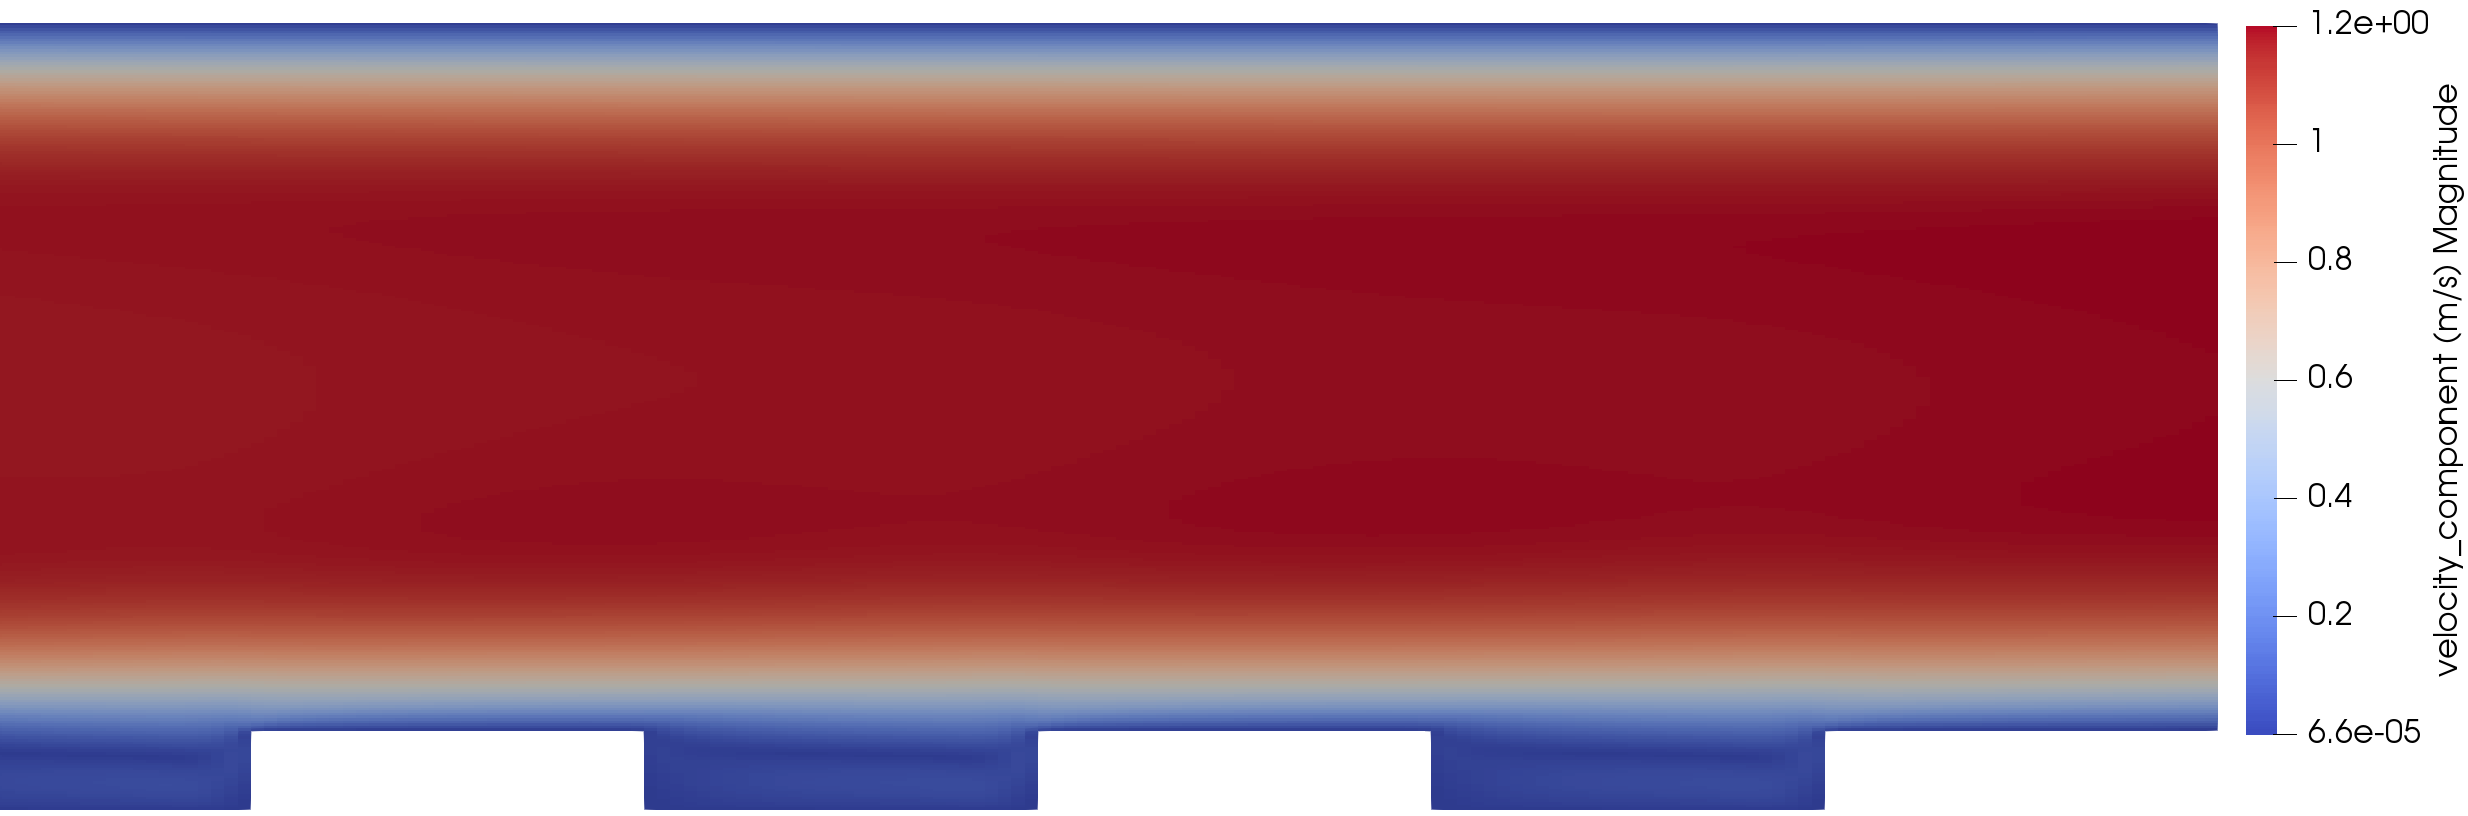
\includegraphics[width=\textwidth]{rough_channel_end}
	\caption{Velocity magnitude at $t=\SI{10}{s}$, $Re=2000$, reference 
	solution.}
	\label{fig:cha_end}
\end{figure}

\begin{table}[h]
	\scriptsize
	\centering
	\[
	\begin{array}{cccccc}
	\toprule
	\text{Upwind} & \text{Van Leer} & \text{Van Alabada} & \text{MinMod} & 
	\text{Superbee} & \text{McLimiter} \\ 
	\midrule
	1.708 \times 10^{-4} & 9.556 \times 10^{-6} & 1.119 \times 10^{-5} & 1.537 
	\times 10^{-5} & 8.335 \times 10^{-6} & 8.659 \times 10^{-6}\\
	\bottomrule
	\end{array}
	\]
	\caption{$L^2$-errors along a section at $x=8.75$m and $t=10$ at $Re = 
	2000$}
	\label{tab:err}
\end{table}

The Upwind method has of an order of magnitude grater then the other methods. 
The Superbee shows the best result, however during the simulation it required 
more Newton steps to converge at each time iterations, resulting in a higher 
computational time.

\FloatBarrier
\subsection{Second case}
Next we solve the same problem over the domain $\Omega$ depicted in Figure 
\ref{fig:line_comp_highstep}, with square cavities that are deeper then those 
in the previous case. The domain has been extended and so a greater number of 
elements in the vertical direction is used, but the cell size is the same of 
that one in the previous case.
\begin{figure}[h]
	\centering
	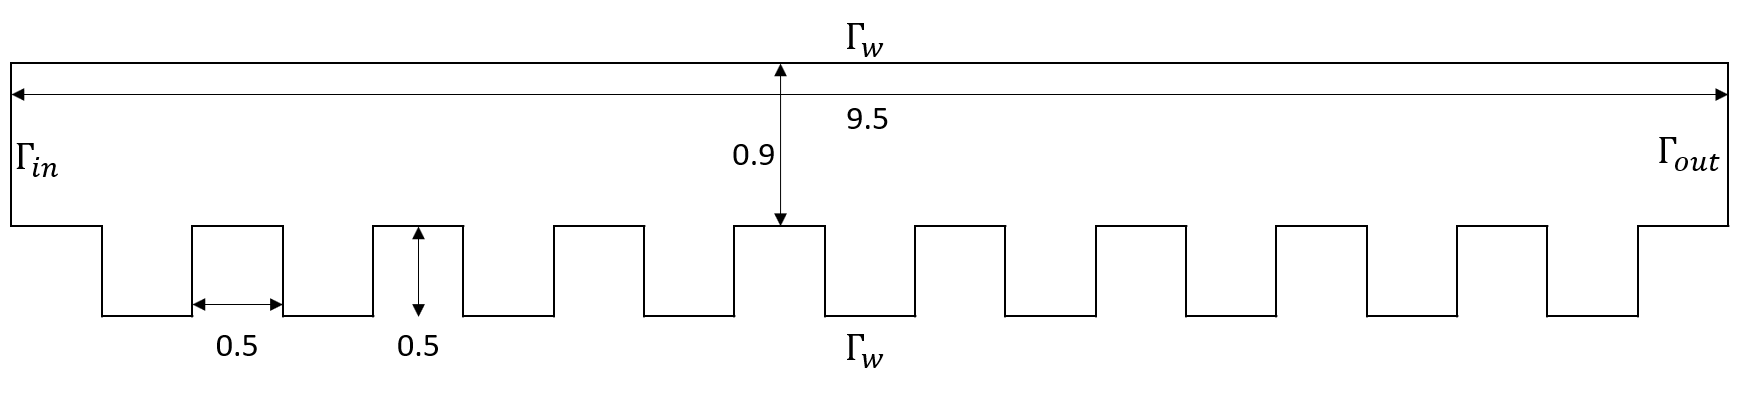
\includegraphics[width = \textwidth]{rough_domain_highstep.png}
	\caption{The domain $\Omega$ with a rough boundary made of deep cavities.}
	\label{fig:rough_domain_highstep}
\end{figure}

In Figure \ref{fig:line_comp_highstep} the magnitude of the velocity along a 
section of the channel at $x=\SI{8.75}{m}$ at the last time step is reported. 
We 
observe a small difference between the upwind the the TVD methods like in the 
previous case, but now there is also a great difference inside the cavity 
($y<\SI{0.5}{m}$). The upwind method has a low of numerical diffusion and the 
variations in the velocity profile related to the recirculation in the cavity 
are smoothed down. The TVD methods do not match exactly the reference solution 
but the result is more accurate. Moreover we have to remember that this portion 
of the domain is of crucial importance in coupled problem because the velocity 
at the interface is responsible for the exchange processes that occur.
\begin{figure}[h]
	\centering
	% This file was created by matlab2tikz.
%
\definecolor{mycolor1}{rgb}{0.00000,0.44700,0.74100}%
\definecolor{mycolor2}{rgb}{0.85000,0.32500,0.09800}%
\definecolor{mycolor3}{rgb}{0.92900,0.69400,0.12500}%
\definecolor{mycolor4}{rgb}{0.49400,0.18400,0.55600}%
%
\begin{tikzpicture}

\begin{axis}[%
width=0.951\roughwidth,
height=0.75\roughheight,
at={(0\roughwidth,0\roughheight)},
scale only axis,
xmin=0,
xmax=1.4,
xlabel={$y$ [m]},
ymin=0,
ymax=1.25,
ylabel={Velocity magnitude [m/s]},
axis background/.style={fill=white},
legend style={at={(0.03,0.97)}, anchor=north west, legend cell align=left, align=left, font=\scriptsize}
]

\addplot [color=mycolor1, mark size=1.5pt, mark=x, mark options={solid, mycolor1}]
  table[row sep=crcr]{%
0	0\\
0.01	0.00885222\\
0.03	0.0227802\\
0.05	0.0327807\\
0.07	0.0393192\\
0.09	0.043122\\
0.11	0.0448784\\
0.13	0.0451341\\
0.15	0.0442874\\
0.17	0.0426208\\
0.19	0.0403378\\
0.21	0.037597\\
0.23	0.0345472\\
0.25	0.0313691\\
0.27	0.0283253\\
0.29	0.0258075\\
0.31	0.0243184\\
0.33	0.024277\\
0.35	0.0257093\\
0.37	0.0283224\\
0.39	0.0319839\\
0.41	0.0370173\\
0.43	0.044611\\
0.45	0.0576046\\
0.47	0.0818451\\
0.49	0.128213\\
0.51	0.214615\\
0.53	0.35431\\
0.55	0.509962\\
0.57	0.654372\\
0.59	0.77967\\
0.61	0.885193\\
0.63	0.971543\\
0.65	1.03985\\
0.67	1.0919\\
0.69	1.12994\\
0.71	1.15654\\
0.73	1.17426\\
0.75	1.18543\\
0.77	1.19201\\
0.79	1.19557\\
0.81	1.19723\\
0.83	1.1978\\
0.85	1.19779\\
0.87	1.19754\\
0.89	1.19723\\
0.91	1.19698\\
0.93	1.19685\\
0.95	1.19686\\
0.97	1.19703\\
0.99	1.19736\\
1.01	1.19783\\
1.03	1.19841\\
1.05	1.19906\\
1.07	1.19964\\
1.09	1.19992\\
1.11	1.19953\\
1.13	1.19783\\
1.15	1.19384\\
1.17	1.1861\\
1.19	1.17264\\
1.21	1.15086\\
1.23	1.11762\\
1.25	1.06938\\
1.27	1.00254\\
1.29	0.913831\\
1.31	0.800848\\
1.33	0.662508\\
1.35	0.499366\\
1.37	0.313659\\
1.39	0.109156\\
1.4	0\\
};
\addlegendentry{Upwind}

\addplot [color=mycolor2, mark size=1.5pt, mark=x, mark options={solid, mycolor2}]
  table[row sep=crcr]{%
0	0\\
0.01	0.0122335\\
0.03	0.0324848\\
0.05	0.0480886\\
0.07	0.0588624\\
0.09	0.0654371\\
0.11	0.0686113\\
0.13	0.0688211\\
0.15	0.0669287\\
0.17	0.0627025\\
0.19	0.0563737\\
0.21	0.0484432\\
0.23	0.0398216\\
0.25	0.0319033\\
0.27	0.0265586\\
0.29	0.0256695\\
0.31	0.0288832\\
0.33	0.0340499\\
0.35	0.0396606\\
0.37	0.0450472\\
0.39	0.0499693\\
0.41	0.0545328\\
0.43	0.0595794\\
0.45	0.0677895\\
0.47	0.0859627\\
0.49	0.128135\\
0.51	0.214164\\
0.53	0.35562\\
0.55	0.519342\\
0.57	0.670222\\
0.59	0.798895\\
0.61	0.905422\\
0.63	0.991025\\
0.65	1.05726\\
0.67	1.10635\\
0.69	1.14101\\
0.71	1.16412\\
0.73	1.17855\\
0.75	1.18688\\
0.77	1.19113\\
0.79	1.19289\\
0.81	1.19325\\
0.83	1.1929\\
0.85	1.19227\\
0.87	1.19163\\
0.89	1.19106\\
0.91	1.19067\\
0.93	1.19044\\
0.95	1.19037\\
0.97	1.1905\\
0.99	1.19084\\
1.01	1.19135\\
1.03	1.19204\\
1.05	1.19284\\
1.07	1.19365\\
1.09	1.19427\\
1.11	1.19434\\
1.13	1.19322\\
1.15	1.1899\\
1.17	1.18285\\
1.19	1.16996\\
1.21	1.14851\\
1.23	1.11525\\
1.25	1.06662\\
1.27	0.999152\\
1.29	0.909811\\
1.31	0.796478\\
1.33	0.658286\\
1.35	0.495815\\
1.37	0.311267\\
1.39	0.108298\\
1.4	0\\
};
\addlegendentry{Van Leer}

\addplot [color=mycolor3, mark size=1.5pt, mark=x, mark options={solid, mycolor3}]
  table[row sep=crcr]{%
0	0\\
0.01	0.0113419\\
0.03	0.0297822\\
0.05	0.0438459\\
0.07	0.0535293\\
0.09	0.0594514\\
0.11	0.0623285\\
0.13	0.0627341\\
0.15	0.0613312\\
0.17	0.0581295\\
0.19	0.0533229\\
0.21	0.0472654\\
0.23	0.040544\\
0.25	0.0340756\\
0.27	0.0291588\\
0.29	0.0272168\\
0.31	0.0284915\\
0.33	0.0317763\\
0.35	0.0359173\\
0.37	0.0402998\\
0.39	0.0446982\\
0.41	0.0493064\\
0.43	0.0551453\\
0.45	0.0648297\\
0.47	0.0848545\\
0.49	0.128268\\
0.51	0.214524\\
0.53	0.355773\\
0.55	0.518594\\
0.57	0.668691\\
0.59	0.796856\\
0.61	0.903066\\
0.63	0.988544\\
0.65	1.05485\\
0.67	1.10418\\
0.69	1.13918\\
0.71	1.16273\\
0.73	1.17764\\
0.75	1.1864\\
0.77	1.19104\\
0.79	1.19311\\
0.81	1.19369\\
0.83	1.19352\\
0.85	1.19301\\
0.87	1.19243\\
0.89	1.19193\\
0.91	1.19158\\
0.93	1.19138\\
0.95	1.19133\\
0.97	1.19148\\
0.99	1.19181\\
1.01	1.19232\\
1.03	1.19298\\
1.05	1.19375\\
1.07	1.19452\\
1.09	1.19508\\
1.11	1.19505\\
1.13	1.19379\\
1.15	1.1903\\
1.17	1.18309\\
1.19	1.17005\\
1.21	1.14852\\
1.23	1.11526\\
1.25	1.06673\\
1.27	0.999415\\
1.29	0.910241\\
1.31	0.797042\\
1.33	0.658892\\
1.35	0.496348\\
1.37	0.311635\\
1.39	0.108434\\
1.4	0\\
};
\addlegendentry{Min-Mod}

\addplot [color=mycolor4]
  table[row sep=crcr]{%
0	0\\
0.00166667	0.00162965\\
0.005	0.00480799\\
0.00833333	0.00790634\\
0.0116667	0.0109252\\
0.015	0.013865\\
0.0183333	0.0167258\\
0.0216667	0.019508\\
0.025	0.022212\\
0.0283333	0.0248383\\
0.0316667	0.0273878\\
0.035	0.0298613\\
0.0383333	0.03226\\
0.0416667	0.0345853\\
0.045	0.0368385\\
0.0483333	0.0390211\\
0.0516667	0.0411348\\
0.055	0.0431809\\
0.0583333	0.045161\\
0.0616667	0.0470764\\
0.065	0.0489283\\
0.0683333	0.0507176\\
0.0716667	0.0524452\\
0.075	0.0541115\\
0.0783333	0.055717\\
0.0816667	0.0572619\\
0.085	0.0587457\\
0.0883333	0.0601683\\
0.0916667	0.0615291\\
0.095	0.0628271\\
0.0983333	0.0640617\\
0.101667	0.0652316\\
0.105	0.0663357\\
0.108333	0.0673728\\
0.111667	0.0683414\\
0.115	0.0692403\\
0.118333	0.070068\\
0.121667	0.0708231\\
0.125	0.0715044\\
0.128333	0.0721104\\
0.131667	0.0726401\\
0.135	0.0730923\\
0.138333	0.0734658\\
0.141667	0.0737601\\
0.145	0.0739741\\
0.148333	0.0741073\\
0.151667	0.0741594\\
0.155	0.0741298\\
0.158333	0.0740188\\
0.161667	0.0738262\\
0.165	0.0735523\\
0.168333	0.0731975\\
0.171667	0.0727624\\
0.175	0.0722478\\
0.178333	0.0716544\\
0.181667	0.0709837\\
0.185	0.0702367\\
0.188333	0.0694149\\
0.191667	0.0685199\\
0.195	0.0675533\\
0.198333	0.0665172\\
0.201667	0.0654135\\
0.205	0.0642444\\
0.208333	0.0630124\\
0.211667	0.0617197\\
0.215	0.0603692\\
0.218333	0.0589636\\
0.221667	0.0575058\\
0.225	0.055999\\
0.228333	0.0544466\\
0.231667	0.0528522\\
0.235	0.0512197\\
0.238333	0.0495534\\
0.241667	0.0478579\\
0.245	0.0461384\\
0.248333	0.0444006\\
0.251667	0.042651\\
0.255	0.0408971\\
0.258333	0.0391474\\
0.261667	0.0374118\\
0.265	0.0357016\\
0.268333	0.0340304\\
0.271667	0.032414\\
0.275	0.0308707\\
0.278333	0.0294217\\
0.281667	0.0280915\\
0.285	0.026907\\
0.288333	0.025897\\
0.291667	0.0250911\\
0.295	0.0245166\\
0.298333	0.0241958\\
0.301667	0.0241434\\
0.305	0.024363\\
0.308333	0.0248475\\
0.311667	0.0255795\\
0.315	0.0265348\\
0.318333	0.0276856\\
0.321667	0.0290029\\
0.325	0.0304586\\
0.328333	0.0320267\\
0.331667	0.0336841\\
0.335	0.0354105\\
0.338333	0.0371883\\
0.341667	0.0390024\\
0.345	0.0408399\\
0.348333	0.0426898\\
0.351667	0.0445425\\
0.355	0.04639\\
0.358333	0.048225\\
0.361667	0.0500416\\
0.365	0.0518343\\
0.368333	0.0535986\\
0.371667	0.0553303\\
0.375	0.0570259\\
0.378333	0.0586824\\
0.381667	0.060297\\
0.385	0.0618676\\
0.388333	0.0633923\\
0.391667	0.0648697\\
0.395	0.0662986\\
0.398333	0.0676785\\
0.401667	0.0690093\\
0.405	0.0702916\\
0.408333	0.0715265\\
0.411667	0.072716\\
0.415	0.0738628\\
0.418333	0.0749713\\
0.421667	0.076047\\
0.425	0.0770969\\
0.428333	0.0781306\\
0.431667	0.0791597\\
0.435	0.0801992\\
0.438333	0.0812674\\
0.441667	0.0823869\\
0.445	0.0835853\\
0.448333	0.084896\\
0.451667	0.0863585\\
0.455	0.08802\\
0.458333	0.0899355\\
0.461667	0.0921692\\
0.465	0.0947941\\
0.468333	0.0978929\\
0.471667	0.101558\\
0.475	0.105891\\
0.478333	0.111\\
0.481667	0.117001\\
0.485	0.124015\\
0.488333	0.13216\\
0.491667	0.141554\\
0.495	0.152307\\
0.498333	0.164518\\
0.501667	0.178267\\
0.505	0.193612\\
0.508333	0.210581\\
0.511667	0.229172\\
0.515	0.249346\\
0.518333	0.271026\\
0.521667	0.294097\\
0.525	0.318416\\
0.528333	0.3438\\
0.531667	0.370031\\
0.535	0.396864\\
0.538333	0.42408\\
0.541667	0.451482\\
0.545	0.478885\\
0.548333	0.506133\\
0.551667	0.533085\\
0.555	0.559629\\
0.558333	0.585678\\
0.561667	0.611162\\
0.565	0.636036\\
0.568333	0.660269\\
0.571667	0.683845\\
0.575	0.706758\\
0.578333	0.729008\\
0.581667	0.750601\\
0.585	0.771545\\
0.588333	0.79185\\
0.591667	0.811525\\
0.595	0.83058\\
0.598333	0.849024\\
0.601667	0.866863\\
0.605	0.884107\\
0.608333	0.900759\\
0.611667	0.916826\\
0.615	0.932313\\
0.618333	0.947225\\
0.621667	0.961569\\
0.625	0.975348\\
0.628333	0.988573\\
0.631667	1.00125\\
0.635	1.01338\\
0.638333	1.02498\\
0.641667	1.03605\\
0.645	1.04661\\
0.648333	1.05667\\
0.651667	1.06623\\
0.655	1.07531\\
0.658333	1.08392\\
0.661667	1.09207\\
0.665	1.09978\\
0.668333	1.10705\\
0.671667	1.11391\\
0.675	1.12035\\
0.678333	1.12641\\
0.681667	1.13209\\
0.685	1.1374\\
0.688333	1.14237\\
0.691667	1.147\\
0.695	1.15131\\
0.698333	1.15531\\
0.701667	1.15901\\
0.705	1.16244\\
0.708333	1.1656\\
0.711667	1.16851\\
0.715	1.17118\\
0.718333	1.17363\\
0.721667	1.17586\\
0.725	1.17789\\
0.728333	1.17974\\
0.731667	1.18141\\
0.735	1.18291\\
0.738333	1.18425\\
0.741667	1.18546\\
0.745	1.18653\\
0.748333	1.18747\\
0.751667	1.18831\\
0.755	1.18903\\
0.758333	1.18966\\
0.761667	1.1902\\
0.765	1.19066\\
0.768333	1.19104\\
0.771667	1.19135\\
0.775	1.19161\\
0.778333	1.19181\\
0.781667	1.19195\\
0.785	1.19206\\
0.788333	1.19212\\
0.791667	1.19214\\
0.795	1.19214\\
0.798333	1.19211\\
0.801667	1.19205\\
0.805	1.19197\\
0.808333	1.19188\\
0.811667	1.19177\\
0.815	1.19164\\
0.818333	1.19151\\
0.821667	1.19136\\
0.825	1.19121\\
0.828333	1.19106\\
0.831667	1.1909\\
0.835	1.19073\\
0.838333	1.19057\\
0.841667	1.19041\\
0.845	1.19025\\
0.848333	1.19009\\
0.851667	1.18993\\
0.855	1.18977\\
0.858333	1.18962\\
0.861667	1.18947\\
0.865	1.18933\\
0.868333	1.18919\\
0.871667	1.18906\\
0.875	1.18893\\
0.878333	1.18881\\
0.881667	1.18869\\
0.885	1.18858\\
0.888333	1.18847\\
0.891667	1.18838\\
0.895	1.18828\\
0.898333	1.1882\\
0.901667	1.18812\\
0.905	1.18804\\
0.908333	1.18797\\
0.911667	1.18791\\
0.915	1.18786\\
0.918333	1.18781\\
0.921667	1.18776\\
0.925	1.18773\\
0.928333	1.1877\\
0.931667	1.18767\\
0.935	1.18765\\
0.938333	1.18764\\
0.941667	1.18763\\
0.945	1.18763\\
0.948333	1.18764\\
0.951667	1.18765\\
0.955	1.18767\\
0.958333	1.18769\\
0.961667	1.18772\\
0.965	1.18776\\
0.968333	1.1878\\
0.971667	1.18785\\
0.975	1.1879\\
0.978333	1.18797\\
0.981667	1.18803\\
0.985	1.18811\\
0.988333	1.18818\\
0.991667	1.18827\\
0.995	1.18836\\
0.998333	1.18846\\
1.00167	1.18856\\
1.005	1.18867\\
1.00833	1.18879\\
1.01167	1.18891\\
1.015	1.18904\\
1.01833	1.18917\\
1.02167	1.18931\\
1.025	1.18946\\
1.02833	1.18961\\
1.03167	1.18977\\
1.035	1.18993\\
1.03833	1.1901\\
1.04167	1.19027\\
1.045	1.19045\\
1.04833	1.19063\\
1.05167	1.19081\\
1.055	1.191\\
1.05833	1.19119\\
1.06167	1.19139\\
1.065	1.19158\\
1.06833	1.19177\\
1.07167	1.19197\\
1.075	1.19216\\
1.07833	1.19235\\
1.08167	1.19253\\
1.085	1.19271\\
1.08833	1.19288\\
1.09167	1.19305\\
1.095	1.1932\\
1.09833	1.19333\\
1.10167	1.19345\\
1.105	1.19355\\
1.10833	1.19362\\
1.11167	1.19367\\
1.115	1.19369\\
1.11833	1.19368\\
1.12167	1.19363\\
1.125	1.19353\\
1.12833	1.19338\\
1.13167	1.19319\\
1.135	1.19293\\
1.13833	1.1926\\
1.14167	1.1922\\
1.145	1.19172\\
1.14833	1.19115\\
1.15167	1.19049\\
1.155	1.18971\\
1.15833	1.18883\\
1.16167	1.18782\\
1.165	1.18667\\
1.16833	1.18538\\
1.17167	1.18393\\
1.175	1.18231\\
1.17833	1.18051\\
1.18167	1.17852\\
1.185	1.17632\\
1.18833	1.17389\\
1.19167	1.17123\\
1.195	1.16832\\
1.19833	1.16515\\
1.20167	1.1617\\
1.205	1.15794\\
1.20833	1.15388\\
1.21167	1.14949\\
1.215	1.14475\\
1.21833	1.13965\\
1.22167	1.13417\\
1.225	1.12829\\
1.22833	1.12201\\
1.23167	1.11529\\
1.235	1.10812\\
1.23833	1.1005\\
1.24167	1.09239\\
1.245	1.08378\\
1.24833	1.07466\\
1.25167	1.06502\\
1.255	1.05483\\
1.25833	1.04408\\
1.26167	1.03276\\
1.265	1.02085\\
1.26833	1.00835\\
1.27167	0.995228\\
1.275	0.981485\\
1.27833	0.967108\\
1.28167	0.952085\\
1.285	0.936409\\
1.28833	0.92007\\
1.29167	0.903062\\
1.295	0.885377\\
1.29833	0.867011\\
1.30167	0.847959\\
1.305	0.828218\\
1.30833	0.807786\\
1.31167	0.786662\\
1.315	0.764846\\
1.31833	0.742339\\
1.32167	0.719144\\
1.325	0.695264\\
1.32833	0.670704\\
1.33167	0.645471\\
1.335	0.619571\\
1.33833	0.593012\\
1.34167	0.565805\\
1.345	0.537959\\
1.34833	0.509487\\
1.35167	0.480401\\
1.355	0.450714\\
1.35833	0.420443\\
1.36167	0.389601\\
1.365	0.358207\\
1.36833	0.326277\\
1.37167	0.29383\\
1.375	0.260885\\
1.37833	0.227463\\
1.38167	0.193583\\
1.385	0.159268\\
1.38833	0.124538\\
1.39167	0.0894149\\
1.395	0.0539223\\
1.39833	0.0180823\\
1.4	0\\
};
\addlegendentry{Reference}
\addplot [color=black, dashed]
  table[row sep=crcr]{%
0.5	0\\
0.5 1.25\\
};
\end{axis}
\end{tikzpicture}%
	\caption{Velocity magnitude at $ x = \SI{8.75}{m}$ at $Re = 2000$ with deep 
	cavities}
	\label{fig:line_comp_highstep}
\end{figure}

\begin{figure}[h]
	\centering
	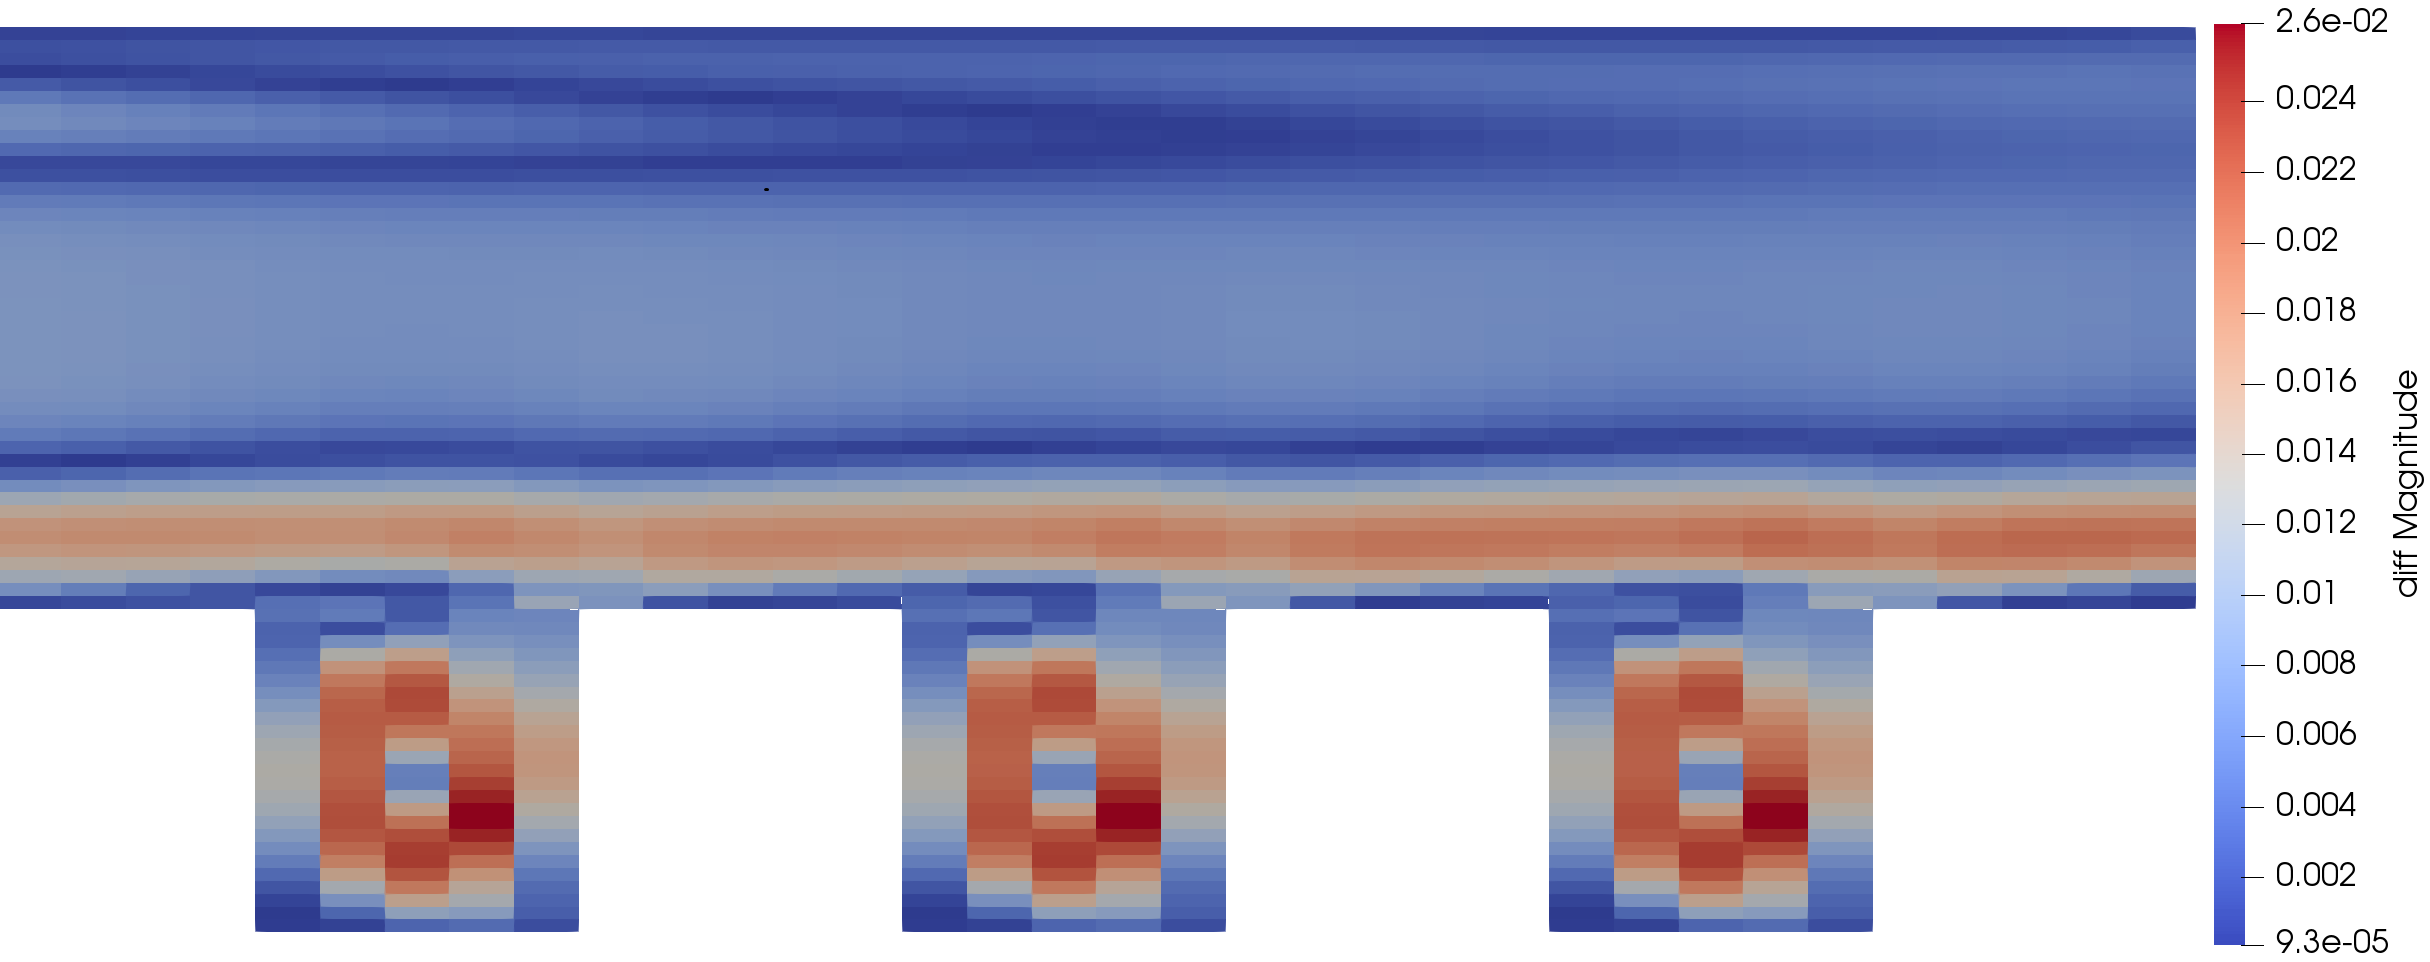
\includegraphics[width=\textwidth]{rough_channel_high_diff}
	\caption{Absolute value of the difference between the magnitude of the 
	velocities obtained with the Upwind and Van Leer methods. $Re = 2000$,
	deep cavities.}
	\label{fig:cha_diff}
\end{figure}

\begin{table}[h]
	\scriptsize
	\centering
	\[
	\begin{array}{cccccc}
	\toprule
	\text{Upwind} & \text{Van Leer} & \text{Van Alabada} & \text{MinMod} & 
	\text{Superbee} & \text{McLimiter} \\ 
	\midrule
	3.180 \times 10^{-4} & 5.862 \times 10^{-5} & 6.900 \times 10^{-5} & 8.579 
	\times 10^{-5} & 7.883 \times 10^{-5} & 5.584 \times 10^{-5}\\
	\bottomrule
	\end{array}
	\]
	\caption{$L^2$-errors along a section at $x=\SI{8.75}{m}$ at $Re = 2000$ 
	with deep cavities}
	\label{tab:err_high}
\end{table}

\FloatBarrier
\subsection{Third case}

In this third case we solve the same problem over the domain $\Omega$ with 
small cavities (Figure \ref{fig:rough_domain}), but at $Re=1$, choosing an 
higher 
viscosity $\mu=\SI{1}{\pascal\second}$. At this regime we observe from Figure 
\ref{fig:line_comp_lre} and Table \ref{tab:err_lre} that the results are the 
same for all the methods. Moreover we observe from the velocity profile that 
there is not the usual recirculation in the cavities.
\begin{figure}[h]
	\centering
	% This file was created by matlab2tikz.
%
\definecolor{mycolor1}{rgb}{0.00000,0.44700,0.74100}%
\definecolor{mycolor2}{rgb}{0.85000,0.32500,0.09800}%
\definecolor{mycolor3}{rgb}{0.92900,0.69400,0.12500}%
\definecolor{mycolor4}{rgb}{0.49400,0.18400,0.55600}%
%
\begin{tikzpicture}

\begin{axis}[%
width=0.951\roughwidth,
height=0.75\roughheight,
at={(0\roughwidth,0\roughheight)},
scale only axis,
xmin=0,
xmax=1,
xlabel={$y$ [m]},
ymin=0,
ymax=1.5,
ylabel={Velocity magnitude [m/s]},
axis background/.style={fill=white},
legend style={at={(0.5,0.03)}, anchor=south, legend cell align=left, align=left}
]
\addplot [color=mycolor1, mark size=1.5pt, mark=x, mark options={solid, mycolor1}]
  table[row sep=crcr]{%
0	0\\
0.01	0.0254229\\
0.03	0.0771412\\
0.05	0.131431\\
0.07	0.189545\\
0.09	0.252263\\
0.11	0.319795\\
0.13	0.391594\\
0.15	0.466634\\
0.17	0.543711\\
0.19	0.621626\\
0.21	0.699267\\
0.23	0.775657\\
0.25	0.849957\\
0.27	0.921463\\
0.29	0.989594\\
0.31	1.05388\\
0.33	1.11392\\
0.35	1.16942\\
0.37	1.22012\\
0.39	1.26583\\
0.41	1.3064\\
0.43	1.34169\\
0.45	1.37161\\
0.47	1.39609\\
0.49	1.41506\\
0.51	1.42849\\
0.53	1.43632\\
0.55	1.43854\\
0.57	1.43512\\
0.59	1.42606\\
0.61	1.41134\\
0.63	1.39096\\
0.65	1.36491\\
0.67	1.3332\\
0.69	1.29582\\
0.71	1.25279\\
0.73	1.2041\\
0.75	1.14977\\
0.77	1.0898\\
0.79	1.02421\\
0.81	0.953007\\
0.83	0.876208\\
0.85	0.79383\\
0.87	0.705892\\
0.89	0.612418\\
0.91	0.513432\\
0.93	0.408963\\
0.95	0.299044\\
0.97	0.183712\\
0.99	0.063011\\
1	0\\
};
\addlegendentry{Upwind}

\addplot [color=mycolor2, mark size=1.5pt, mark=x, mark options={solid, mycolor2}]
  table[row sep=crcr]{%
0	0\\
0.01	0.0256098\\
0.03	0.0776368\\
0.05	0.132183\\
0.07	0.190504\\
0.09	0.253384\\
0.11	0.321031\\
0.13	0.392898\\
0.15	0.467961\\
0.17	0.54502\\
0.19	0.62289\\
0.21	0.700459\\
0.23	0.77675\\
0.25	0.850931\\
0.27	0.922307\\
0.29	0.990298\\
0.31	1.05443\\
0.33	1.11433\\
0.35	1.16969\\
0.37	1.22025\\
0.39	1.26584\\
0.41	1.30628\\
0.43	1.34146\\
0.45	1.37129\\
0.47	1.39566\\
0.49	1.41456\\
0.51	1.42791\\
0.53	1.43568\\
0.55	1.43786\\
0.57	1.4344\\
0.59	1.42531\\
0.61	1.41057\\
0.63	1.39018\\
0.65	1.36413\\
0.67	1.33242\\
0.69	1.29505\\
0.71	1.25203\\
0.73	1.20336\\
0.75	1.14905\\
0.77	1.08912\\
0.79	1.02356\\
0.81	0.952393\\
0.83	0.875636\\
0.85	0.793306\\
0.87	0.70542\\
0.89	0.612002\\
0.91	0.513077\\
0.93	0.408675\\
0.95	0.298828\\
0.97	0.183576\\
0.99	0.0629624\\
1	0\\
};
\addlegendentry{Van Leer}

\addplot [color=mycolor3, mark size=1.5pt, mark=x, mark options={solid, mycolor3}]
  table[row sep=crcr]{%
0	0\\
0.01	0.0255838\\
0.03	0.0775663\\
0.05	0.132074\\
0.07	0.190362\\
0.09	0.253217\\
0.11	0.320848\\
0.13	0.392711\\
0.15	0.467774\\
0.17	0.544841\\
0.19	0.622723\\
0.21	0.70031\\
0.23	0.776621\\
0.25	0.850825\\
0.27	0.92222\\
0.29	0.990231\\
0.31	1.05439\\
0.33	1.1143\\
0.35	1.16968\\
0.37	1.22026\\
0.39	1.26586\\
0.41	1.30632\\
0.43	1.34151\\
0.45	1.37134\\
0.47	1.39573\\
0.49	1.41463\\
0.51	1.42799\\
0.53	1.43577\\
0.55	1.43795\\
0.57	1.4345\\
0.59	1.42541\\
0.61	1.41067\\
0.63	1.39028\\
0.65	1.36422\\
0.67	1.33251\\
0.69	1.29514\\
0.71	1.25212\\
0.73	1.20345\\
0.75	1.14914\\
0.77	1.08919\\
0.79	1.02363\\
0.81	0.952462\\
0.83	0.8757\\
0.85	0.793364\\
0.87	0.705472\\
0.89	0.612048\\
0.91	0.513116\\
0.93	0.408706\\
0.95	0.298851\\
0.97	0.183591\\
0.99	0.0629675\\
1	0\\
};
\addlegendentry{MinMod}

\addplot [color=mycolor4]
  table[row sep=crcr]{%
0	0\\
0.00166667	0.00452198\\
0.005	0.0135298\\
0.00833333	0.0225133\\
0.0116667	0.0314839\\
0.015	0.0404525\\
0.0183333	0.0494296\\
0.0216667	0.0584251\\
0.025	0.0674484\\
0.0283333	0.0765086\\
0.0316667	0.0856141\\
0.035	0.0947727\\
0.0383333	0.103992\\
0.0416667	0.113279\\
0.045	0.122639\\
0.0483333	0.13208\\
0.0516667	0.141606\\
0.055	0.151223\\
0.0583333	0.160933\\
0.0616667	0.170742\\
0.065	0.180653\\
0.0683333	0.190669\\
0.0716667	0.200792\\
0.075	0.211024\\
0.0783333	0.221367\\
0.0816667	0.231823\\
0.085	0.242391\\
0.0883333	0.253073\\
0.0916667	0.263866\\
0.095	0.274774\\
0.0983333	0.285794\\
0.101667	0.296923\\
0.105	0.308161\\
0.108333	0.319508\\
0.111667	0.330959\\
0.115	0.342513\\
0.118333	0.354168\\
0.121667	0.365919\\
0.125	0.377765\\
0.128333	0.3897\\
0.131667	0.401723\\
0.135	0.413829\\
0.138333	0.426013\\
0.141667	0.438273\\
0.145	0.450603\\
0.148333	0.462999\\
0.151667	0.475457\\
0.155	0.487973\\
0.158333	0.50054\\
0.161667	0.513155\\
0.165	0.525812\\
0.168333	0.538508\\
0.171667	0.551237\\
0.175	0.563993\\
0.178333	0.576772\\
0.181667	0.58957\\
0.185	0.602381\\
0.188333	0.615201\\
0.191667	0.628024\\
0.195	0.640846\\
0.198333	0.653662\\
0.201667	0.666468\\
0.205	0.679258\\
0.208333	0.69203\\
0.211667	0.704776\\
0.215	0.717494\\
0.218333	0.730179\\
0.221667	0.742827\\
0.225	0.755434\\
0.228333	0.767995\\
0.231667	0.780507\\
0.235	0.792966\\
0.238333	0.805369\\
0.241667	0.81771\\
0.245	0.829988\\
0.248333	0.842198\\
0.251667	0.854338\\
0.255	0.866403\\
0.258333	0.878391\\
0.261667	0.890298\\
0.265	0.902123\\
0.268333	0.913861\\
0.271667	0.925509\\
0.275	0.937066\\
0.278333	0.948529\\
0.281667	0.959895\\
0.285	0.971162\\
0.288333	0.982327\\
0.291667	0.993388\\
0.295	1.00434\\
0.298333	1.01519\\
0.301667	1.02593\\
0.305	1.03655\\
0.308333	1.04706\\
0.311667	1.05746\\
0.315	1.06773\\
0.318333	1.07789\\
0.321667	1.08792\\
0.325	1.09784\\
0.328333	1.10763\\
0.331667	1.1173\\
0.335	1.12684\\
0.338333	1.13625\\
0.341667	1.14553\\
0.345	1.15468\\
0.348333	1.1637\\
0.351667	1.17258\\
0.355	1.18133\\
0.358333	1.18995\\
0.361667	1.19843\\
0.365	1.20677\\
0.368333	1.21498\\
0.371667	1.22305\\
0.375	1.23097\\
0.378333	1.23876\\
0.381667	1.24641\\
0.385	1.25391\\
0.388333	1.26127\\
0.391667	1.26849\\
0.395	1.27556\\
0.398333	1.28249\\
0.401667	1.28927\\
0.405	1.29591\\
0.408333	1.3024\\
0.411667	1.30875\\
0.415	1.31495\\
0.418333	1.321\\
0.421667	1.3269\\
0.425	1.33266\\
0.428333	1.33826\\
0.431667	1.34372\\
0.435	1.34902\\
0.438333	1.35417\\
0.441667	1.35918\\
0.445	1.36403\\
0.448333	1.36873\\
0.451667	1.37328\\
0.455	1.37768\\
0.458333	1.38191\\
0.461667	1.38601\\
0.465	1.38995\\
0.468333	1.39373\\
0.471667	1.39737\\
0.475	1.40085\\
0.478333	1.40417\\
0.481667	1.40735\\
0.485	1.41036\\
0.488333	1.41323\\
0.491667	1.41594\\
0.495	1.41849\\
0.498333	1.42089\\
0.501667	1.42313\\
0.505	1.42522\\
0.508333	1.42716\\
0.511667	1.42894\\
0.515	1.43056\\
0.518333	1.43202\\
0.521667	1.43334\\
0.525	1.43449\\
0.528333	1.43549\\
0.531667	1.43633\\
0.535	1.43702\\
0.538333	1.43755\\
0.541667	1.43792\\
0.545	1.43814\\
0.548333	1.4382\\
0.551667	1.4381\\
0.555	1.43785\\
0.558333	1.43744\\
0.561667	1.43687\\
0.565	1.43615\\
0.568333	1.43527\\
0.571667	1.43423\\
0.575	1.43304\\
0.578333	1.43168\\
0.581667	1.43017\\
0.585	1.4285\\
0.588333	1.42668\\
0.591667	1.4247\\
0.595	1.42256\\
0.598333	1.42026\\
0.601667	1.41781\\
0.605	1.4152\\
0.608333	1.41243\\
0.611667	1.40951\\
0.615	1.40642\\
0.618333	1.40319\\
0.621667	1.39979\\
0.625	1.39623\\
0.628333	1.39252\\
0.631667	1.38865\\
0.635	1.38462\\
0.638333	1.38044\\
0.641667	1.3761\\
0.645	1.3716\\
0.648333	1.36694\\
0.651667	1.36213\\
0.655	1.35715\\
0.658333	1.35202\\
0.661667	1.34674\\
0.665	1.34129\\
0.668333	1.33569\\
0.671667	1.32993\\
0.675	1.32402\\
0.678333	1.31794\\
0.681667	1.31171\\
0.685	1.30532\\
0.688333	1.29878\\
0.691667	1.29207\\
0.695	1.28521\\
0.698333	1.2782\\
0.701667	1.27102\\
0.705	1.26369\\
0.708333	1.2562\\
0.711667	1.24855\\
0.715	1.24075\\
0.718333	1.23279\\
0.721667	1.22467\\
0.725	1.2164\\
0.728333	1.20797\\
0.731667	1.19938\\
0.735	1.19064\\
0.738333	1.18174\\
0.741667	1.17268\\
0.745	1.16346\\
0.748333	1.15409\\
0.751667	1.14456\\
0.755	1.13488\\
0.758333	1.12504\\
0.761667	1.11504\\
0.765	1.10489\\
0.768333	1.09458\\
0.771667	1.08411\\
0.775	1.07349\\
0.778333	1.06271\\
0.781667	1.05177\\
0.785	1.04068\\
0.788333	1.02943\\
0.791667	1.01803\\
0.795	1.00647\\
0.798333	0.994758\\
0.801667	0.982888\\
0.805	0.970862\\
0.808333	0.958681\\
0.811667	0.946344\\
0.815	0.933851\\
0.818333	0.921203\\
0.821667	0.9084\\
0.825	0.895442\\
0.828333	0.882328\\
0.831667	0.86906\\
0.835	0.855636\\
0.838333	0.842058\\
0.841667	0.828325\\
0.845	0.814438\\
0.848333	0.800395\\
0.851667	0.786198\\
0.855	0.771847\\
0.858333	0.757342\\
0.861667	0.742682\\
0.865	0.727868\\
0.868333	0.712901\\
0.871667	0.697779\\
0.875	0.682504\\
0.878333	0.667075\\
0.881667	0.651492\\
0.885	0.635756\\
0.888333	0.619867\\
0.891667	0.603825\\
0.895	0.587629\\
0.898333	0.571281\\
0.901667	0.55478\\
0.905	0.538126\\
0.908333	0.521319\\
0.911667	0.504361\\
0.915	0.48725\\
0.918333	0.469987\\
0.921667	0.452572\\
0.925	0.435005\\
0.928333	0.417287\\
0.931667	0.399417\\
0.935	0.381396\\
0.938333	0.363224\\
0.941667	0.344901\\
0.945	0.326427\\
0.948333	0.307803\\
0.951667	0.289028\\
0.955	0.270103\\
0.958333	0.251028\\
0.961667	0.231803\\
0.965	0.212428\\
0.968333	0.192904\\
0.971667	0.173231\\
0.975	0.153409\\
0.978333	0.133438\\
0.981667	0.113319\\
0.985	0.0930514\\
0.988333	0.0726357\\
0.991667	0.0520722\\
0.995	0.0313611\\
0.998333	0.0105027\\
1	0\\
};
\addlegendentry{Reference}
\addplot [color=black, dashed]
  table[row sep=crcr]{%
0.1	0\\
0.1 1.5\\
};
\end{axis}
\end{tikzpicture}%
	\caption{Velocity magnitude at $ x = \SI{8.75}{m}$ at $Re = 1$}
	\label{fig:line_comp_lre}
\end{figure}

\begin{table}[h]
	\scriptsize
	\centering
	\[
	\begin{array}{cccccc}
	\toprule
	\text{Upwind} & \text{Van Leer} & \text{Van Alabada} & \text{MinMod} & 
	\text{Superbee} & \text{McLimiter} \\ 
	\midrule
	3.431 \times 10^{-6} & 2.917 \times 10^{-6} & 2.937 \times 10^{-6} & 2.956 
	\times 10^{-6} & 2.899 \times 10^{-6} & 2.902 \times 10^{-6}\\
	\bottomrule
	\end{array}
	\]
	\caption{$L^2$-errors along a section at $x=\SI{8.75}{m}$ at $Re=1$}
	\label{tab:err_lre}
\end{table}

\FloatBarrier

\section{RANS test}
We would like to perform the test over the domain $\Omega$ at higher $Re$, 
employing a RANS model to take into account the effect of turbulence that would 
be lost with the Navier-Stokes model.\\
The available turbulence models in \DUMUX are:
\begin{itemize}
	\item Algebraic models that exploit the mixing length concept: Prandtl, Van 
	Driest, Baldwin-Lomax. They compute the turbulent viscosity $\nu_t$ without 
	any additional PDE, so they are a cheap choice, but they have been 
	developed in order to solve simple situations with flat walls, but our case 
	such a simple one.
	\item The Spalart-Allmaras one equation model that uses one PDE to compute 
	the evolution of a variable $\tilde{\nu}$ that is proportional to the 
	turbulent viscosity $\nu_t$.
	\item Two equations models: $k$-$\varepsilon$, low-$Re$ $k$-$\varepsilon$, 
	$k$-$\omega$. The $k$-$\varepsilon$ model exploits a wall law in order for 
	the approximation of the velocities near the boundaries. Since our lower 
	boundary is not flat, the straight forwards application of the wall law 
	could produce wrong results. It is better to rely on the low-$Re$ 
	$k$-$\varepsilon$ and $k$-$\omega$ models that solve the evolution 
	equations in the whole domain.
\end{itemize}
%
The equations needed by the RANS model are independent of the TVD 
discretization that we have adopted for the momentum equation because they are 
discretized using a cell-centred grid.

\section{Conclusions}
\begin{thebibliography}{99}\label{sec:bib}
	
	\bibitem{fetzer} T. Fetzer. \emph{Coupled Free and Porous-Medium Flow 
	Processes Affected by Turbulence and Roughness}. PhD thesis, Universit\"at 
	Stuttgart, 2018.
	
	\bibitem{pope} S. B. Pope. \emph{Turbulent Flows}. Cambridge University 
	Press, 2006.
	
\end{thebibliography}

\end{document}